% -------------------------------------------------------------------------------- %

\begin{exercise}[Confidence interval 1]

In the June 1981 issue of Consumer Reports, some data on the calorie content of beef hot dogs is given.
Here are the numbers of calories in $20$ different hot dog brands:

\begin{align*}
    186, 181, 176, 149, 184, 190, 158, 139, 175, 148, 152, 111, 141, 153, 190, 157, 131, 149, 135, 132.
\end{align*}

Assume that the numbers are from a normal distribution with mean $\mu$ and variance $\sigma^2$, both unknown.
Use \texttt R to obtain a $90 \%$ confidence interval for the mean number of calories $\mu$.

\end{exercise}

% -------------------------------------------------------------------------------- %

\begin{solution}

\phantom{}

\includepdf[
    pages = {16},
    nup = 1x2
]
{../../../EStat_VO/Lecture Slides/Lecture 9.pdf}

\lstinputlisting{10.2.r}

\end{solution}

% -------------------------------------------------------------------------------- %
